

\documentclass{article}
\usepackage[final]{graphicx}
\usepackage{caption}
\usepackage{subcaption}
\usepackage[utf8]{inputenc}
\usepackage{amsmath}
\usepackage{amssymb}
\usepackage{anysize}
\usepackage{color}
\usepackage{xcolor}
\usepackage{algpseudocode}
\usepackage[framed,numbered,autolinebreaks,useliterate]{mcode}
\usepackage{floatrow}


\usepackage{algorithmicx}
\usepackage[]{algorithm2e}


\usepackage{listings}
\lstset{
	language=Matlab,                	% choose the language of the code
	basicstyle=\footnotesize,       % the size of the fonts that are used for the code
	numbers= left,                 	% where to put the line-numbers
	numberstyle=\footnotesize,      % the size of the fonts that are used for the line-numbers
	stepnumber=2,                   % the step between two line-numbers. If it is 1 each line will be numbered
	numbersep=5pt,                  % how far the line-numbers are from the code
	backgroundcolor=\color{white},  % choose the background color. You must add \usepackage{color}
	showspaces=false,               % show spaces adding particular underscores
	showstringspaces=false,         % underline spaces within strings
	showtabs=false,                 % show tabs within strings adding particular underscores
	frame=single,           		% adds a frame around the code
	tabsize=2,          			% sets default tabsize to 2 spaces
	captionpos=t,          			% sets the caption-position to bottom (t=top, b=bottom)
	breaklines=true,        		% sets automatic line breaking
	breakatwhitespace=false,    	% sets if automatic breaks should only happen at whitespace
	escapeinside={\%*}{*)}          % if you want to add a comment within your code
}



\usepackage{caption}
\DeclareCaptionFont{white}{\color{white}}
\DeclareCaptionFormat{listing}{\colorbox{gray}{\parbox[c]{\textwidth}{#1#2#3}}}
\captionsetup[lstlisting]{format=listing,labelfont=white,textfont=white}

\setlength\parindent{0pt}
\setlength{\parskip}{10pt}

\marginsize{3cm}{2cm}{2cm}{2cm}
%\documentclass[12pt]{article}

\begin{document}

\begin{titlepage}

\newcommand{\HRule}{\rule{\linewidth}{0.5mm}} % Defines a new command for the horizontal lines, change thickness here

\center % Center everything on the page
 
%----------------------------------------------------------------------------------------
%	HEADING SECTIONS
%----------------------------------------------------------------------------------------

\textsc{\LARGE Master Computer Vision}\\[1.5cm] % Name of your university/college
\textsc{\Large Scene Segmentation and Interpretation}\\[0.5cm] % Major heading such as course name


%----------------------------------------------------------------------------------------
%	TITLE SECTION
%----------------------------------------------------------------------------------------

\HRule \\[0.4cm]
{ \huge \bfseries Image Segmentation}\\[0.4cm] % Title of your document
\HRule \\[1.5cm]
 
%----------------------------------------------------------------------------------------
%	AUTHOR SECTION
%----------------------------------------------------------------------------------------

\begin{minipage}{0.4\textwidth}
\begin{flushleft} \large
\emph{Author:}\\
Muhammad \textsc{Usman} \\
Emre Ozan \textsc{Alkan}\\
Priyanka \textsc{Phutane}

\end{flushleft}
\end{minipage}
~
\begin{minipage}{0.4\textwidth}
\begin{flushright} \large
\emph{Course Co ordinator:} \\
Pere Ridao \textsc{Smith} % Supervisor's Name
\end{flushright}
\end{minipage}\\[4cm]

% If you don't want a supervisor, uncomment the two lines below and remove the section above
%\Large \emph{Author:}\\
%John \textsc{Smith}\\[3cm] % Your name

%----------------------------------------------------------------------------------------
%	DATE SECTION
%----------------------------------------------------------------------------------------

{\large \today}\\[3cm] % Date, change the \today to a set date if you want to be precise

%----------------------------------------------------------------------------------------
%	LOGO SECTION
%----------------------------------------------------------------------------------------

%\includegraphics{Logo}\\[1cm] % Include a department/university logo - this will require the graphicx package
 
%----------------------------------------------------------------------------------------

\vfill % Fill the rest of the page with whitespace
\end{titlepage}

\section{Introduction and Problem Statement:}
Image segmentation means partitioning image into non overlapped segments, based on certain criteria and union of these segments forms an image. The goal of Image segmentation is to transform our image so that it is become easy to analyse. During segmentation we assign labels to image pixels thus pixels having same labels share same characteristics. The similarity criteria within one segment or region may be texture, colour  or intensity but it should remain constant within one segment(region). Segmentation finds wide variety of application in various fields such as Medical Imaging, Machine Vision, Object Detection and Recognition tasks etc.[1] \\
There are wide variety of segmentation methods available in literature. The most basic method of segmentation is simple thresholding. Some common categories of segmentation methods are methods based on clustering, region growing, Split and Merge etc. In this lab our focus will be on segmenting images using region growing.[1] Region Growing algorithm requires selection of seed points in image and for each seed explore its neighbours to check if they follow similarity or aggregation criteria, if yes, include them into our region. We continue growing our regions like this until no pixel in image remained unassigned to certain region. Region Growing methods are very sensitive to selection of seed points and aggregation criteria so lot of care required in choosing these parameters. Our goal is to segment test images using region growing algorithm and then to compare our results with manually segmented images and tune our algorithm to get best results.

\section{Algorithm Analysis:}
There are many variants of Region Growing Algorithms, most basic algorithm just take set of seeds as input and then for each seed explore neighbourhood and check if they can be added to that region under some aggregation criteria or not and thus by doing so grow regions. This algorithm seems very simple but there are some very important question that need to be answered.[2]
\subsection{Selection of Seed Points?}
Selection of seeds is the most important part in region growing algorithm. There are lot of strategies to select the seed points as stated below. Selection of seed mainly depend upon what we want to segment in image.
\begin{itemize}
  \item[1] We may randomly select seed and grow it until no more pixels fulfil the aggregation criteria and then select another seed randomly from unassigned pixels and keep repeating this process until all the pixels get assigned to some region. This method is useful when image under consideration is of complex nature.
  \item[2] We may manually input the certain number of seeds to algorithm. This can be useful when the image is simple and we want to segment desired regions.
  \item[3] We may utilize image information to select and place seeds appropriately. The strategy we devise is to select the local peaks from the histogram and find corresponding intensity value and then select any pixel of that intensity as seed point. We do this for all local peaks and then if some parts of image left un assigned randomly select seed from them. But this method is useful only in case of simple images.

\end{itemize}
\subsection{Type of Adjacency for Neighbourhood:}
We can choose either eight or four Adjacency for selecting neighbourhood but one thing should be kept while selecting that using eight Adjacency will take more time to process.
\subsection{Aggregation Criteria:}
This is the most important and difficult question to answer. There can be number of ways to select the aggregation criteria. Below we enlisted the criteria we used in our implementations.
\begin{itemize}
  \item[1] The first method can be simply take mean of current region and check if intensity of test pixel is inside range, mean plus minus certain threshold or not. If its inside we add it to our region. This threshold is very important as it decides the sensitivity of aggregation criteria.
  \[ \mu_{c} - X < I_{x} < \mu_{c} + X \]
  Where $ I_{x} $ is our test pixel, X is Threshold to selected empirically and $\mu_{c}$ is mean of current region.
  \item[2] We can also calculate mean and standard deviation of the current region. Now we will add test pixel which is being tested for aggregation criteria if it fulfils given condition.
   \[ \mu_{c} - X\sigma_{c} < I_{x} < \mu_{c} + X\sigma_{c} \]
     Where $ I_{x} $ is our test pixel, X is Threshold to be selected empirically,$\sigma_{c}$,$\mu_{c}$ is standard deviation and mean of current region.
  \item[3] For an RGB image we can find mean and standard deviation of three channels separately and then take mean of all standard deviations and use that value as shown below.
   \[ \mu_{c} - X\sigma_{c} < I_{x} < \mu_{c} + X\sigma_{c} \]
   Where,
   \[\mu_{c} = \frac{\mu_{cr} + \mu_{cg} + \mu_{cb}}{3} \]
   and,
   \[\sigma_{c} = \frac{\sigma_{cr} + \sigma_{cg} + \sigma_{cb}}{3} \]
   $\sigma_{c}$ is average of standard deviation of all channels and $\mu_{c}$ is average of means of all channels.
\end{itemize}
\section{Design and Implementation:}
We used Matlab for implementing and testing our segmentation algorithm. We used queue to explore neighbours. When we explore neighbours of pixel we add them to queue and then we check them against aggregation criteria if they agree we add them to region and remove from queue and repeat this process until our queue goes empty or region reaches its maximum area under the given aggregation criteria.\\
For labelling the regions we create another matrix called region matrix of the same size as original image and when some pixels fulfils the aggregation criteria we label it in region matrix. And this matrix will be used at end as a result of segmentation. Also we will maintained a visited matrix which is also of same size as original image. When ever some pixel is assigned to certain region we will make corresponding pixel in visited matrix 1. We will use eight adjacency in our implementations.\\
\\
Add Pseudo Code here\\

\begin{algorithm}[H]
 \KwData{color or gray scale image.}
 \KwData{neighborhood type as 4 or 8.}
 \KwResult{Color segmented image, binary image and region matrix.}
 Initialize ‘visitedMatrix’ as image size with zeros\;
 Initialize ‘regionMatrix’ as image size with zeros\;
 Initialize ‘currentRegionLabel’ with 1\;
 \While{‘regionMatrix’ have unlabeled region marked as zero}{
  Pick ‘seed’ index from ‘regionMatrix’  with found first zero\;
  \If{‘seed’ is empty}{
   stop the loop\;
   }
   Initialize ‘currentRegion’ matrix with empty matrix\;
   ‘currentRegion’ = ‘currentRegion’ $\cup$ ‘seed’\;
   Mark ‘seed’ as visited in ‘visitedMatrix’ with 1\;
   Mark ‘seed’ with ‘currentRegionLabel’ in ‘regionMatrix’\;
   Initialize ‘threshold’ with mean of standard deviation of image\;
   
	Initialize ‘neighborList’ queue with empty matrix\;
	Initialize ‘addedNeighborList’ queue with empty matrix\;
	
	Add ‘seed’’s 4 or 8 neighbors to ‘neighborList’\;
	 \While{‘neighborList’ is not empty}{
	 	\While{‘neighborList’ is not empty}{
	 		Get and remove ‘neighbor’ from top of ‘neighborList’ queue\;
	 		\eIf{‘neighbor’ is marked as visited in ‘visitedMatrix’}{
  			 	skip rest of the loop\;
   			}{
			    Mark ‘neighbor’ as visited in ‘visitedMatrix’\;
  			}
  			
  			Initialize ‘currentPixel’ with pixel value of ‘neighbor’\;
  			Initialize ‘regionMean’ with mean of ‘currentRegion’\;
  			Initialize ‘diff’ with absolute value of difference between ‘currentPixel’ and ‘regionMean’\;

			  \If{‘diff’ smaller or equal to ‘threshold’}{
			  		‘currentRegion’ = ‘currentRegion’ $\cup$ ‘currentPixel’\;
			  		Mark ‘neighbor’ with ‘currentRegionLabel’ in ‘regionMatrix’\;
			  		Add ‘neighbor’ to ‘addedNeighborList’\;
		     }  			
	 	}
	 	\While{‘addedNeighborList’ is not empty}{
	 		Get and remove ‘addedNeighbor’ from top of ‘addedNeighborList’ queue\;
	 		Add ‘addedNeighbor’’s 4 or 8 neighbors to ‘neighborList’\;
	 	}
	 	Set threshold as 8 * standard deviation of mean of ‘currentRegion’\;
	 }
	 Set ‘currentRegionLabel’ as ‘currentRegionLabel’ + 1;
 }
 \caption{Region Growing Segmentation Algorithm}
\end{algorithm}


\begin{algorithm}[H]
 \KwData{Gray scale ‘image’.}
 \KwResult{Entropy, Contrast, Correlation, Energy and Homogeneity images of the input 'image' .}
 Calculate 'entropyImage' with ‘entropyfilt’ function;
 Initialize ‘windowSize’ with odd number preferably 7 or 9\;
 Initialize ‘windowCenter’ with floor of half of ‘windowSize’\;
 Pad the ‘image’ borders with size of ‘windowCenter’\;
 Initialize ‘offset’ with vector in form of  [0 D], [-D, D], [-D, 0,], [-D, -D]\; 
 Initialize ‘numLevels’ with 8\;
 Initialize ‘symmetric’ with false or true\;
 Initialize ‘contrastImage’ as size of ‘image’ with zeros\; 
 Initialize ‘correlationImage’ as size of ‘image’ with zeros\; 
 Initialize ‘energyImage’ as size of ‘image’ with zeros\; 
 Initialize ‘homogeneityImage’ as size of ‘image’ with zeros\; 
 
 Initialize ‘rows’ and ‘cols’ with ‘image’ size\;
 
 \For{$i\leftarrow (‘windowCenter’ + 1)$ \KwTo $(‘rows’ - ‘windowCenter’)$}
 {
 	 \For{$j\leftarrow (‘windowCenter’ + 1)$ \KwTo $(‘cols’ - ‘windowCenter’)$}
 	 {
 	 	Get ‘subImage’ as size of ‘windowCenter’ from ‘image’ with center $i$ and $j$\;
 	 	Compute ‘GLCM’ with ‘graycomatrix’ function as input ‘subImage’\;
 	 	Compute ‘contrast’, ‘correlation’, ‘energy’ and ‘homogeneity’ with ‘graycoprops’ function as input ‘GLCM’
 	 	Set ‘contrastImage’ pixel($i$, $j$) with ‘contrast’\;
 	 	Set ‘correlationImage’ pixel($i$, $j$) with ‘correlation’;
 	 	Set ‘energyImage’ pixel($i$, $j$) with ‘energy’;
 	 	Set ‘homogeneityImage’ pixel($i$, $j$) with ‘homogeneity’;
 	 }
 }
 
 Remove paddings of ‘image’, ‘contrastImage’, ‘correlationImage’, ‘energyImage’ and ‘homogeneityImage’\;
 
 \caption{GLCM Algorithm}
\end{algorithm}










\begin{algorithm}[H]
 \KwData{Colored  ‘image’.}
 \KwResult{Laws' filter ans statistics  of the input ‘image’ .}
Separate RGB channels of the ‘image’ as  ‘imageR’,  ‘imageG’,  ‘imageB’\;
Initialize ‘imageGray’ with gray level of the  input ‘image’\;
Initialize  ‘hsvImage’ with color conversion from RGB of ‘image’\;
Initialize  ‘hueImage’ from ‘hsvImage’'s first channel\;
Initialize lawsMask with some mask\;

Convolve ‘imageGray’, ‘imageR’, ‘imageG’, ‘imageB’,  and ‘hueImage’ with Laws' mask\;
Show the results\;

Initialize ‘filterSize’ with odd number preferable 7 or 9\;

Find mean of the ‘imageGray’, ‘imageR’, ‘imageG’, ‘imageB’,  and ‘hueImage’\;

Initialize ‘meanOutputImage’ with combination of mean of ‘imageGray’, ‘imageR’, ‘imageG’\;

Show the mean results\;

Find absolute mean of the ‘imageGray’, ‘imageR’, ‘imageG’, ‘imageB’,  and ‘hueImage’\;

Initialize ‘absmeanOutputImage’ with combination of absolute mean of ‘imageGray’, ‘imageR’, ‘imageG’\;

Show the absolute mean results\;

Find standart deviation of the ‘imageGray’, ‘imageR’, ‘imageG’, ‘imageB’,  and ‘hueImage’\;

Initialize ‘stdDevOutputImage’ with combination of standart deviation of ‘imageGray’, ‘imageR’, ‘imageG’\;

Show the standart deviation esults\;

 \caption{Energy Filters Algorithm}
\end{algorithm}






When our algorithm is finished with segmentation we change labels to random colours so that we can visualize our results of segmentation in a better way. TO compare our results with ground truth we convert our segmented result to binary image and find specificity and sensitivity.
\subsection{Functions Developed:}
add detail here
\section{Experimental Results and Analysis}
We have implemented our Algorithm for both grayscale and colour images. Now we will present our results for both separately.
\subsection{Implementation on Grayscale Images:}

my table\\
\begin{table}[h]
    \begin{tabular}{|l|l|l|}
    \hline
    Executed Action       & Probability of                   & Probability of \\ 
                          & ROBOT IS DOCKED                   & ROBOT IS NOT DOCKED \\ \hline
    Initial Guess         & 0.5                                & 0.5                                    \\ \hline
    $u_{t}=$ DOCK INTO STATION & 0.85                                & 0.15                                    \\ \hline
    $z_{t} =$ ROBOT IS DOCKED  & 0.9084                                & 0.0916                                    \\ \hline
    \end{tabular}
\end{table}
\subsection{Solution:}

\begin{figure}[H]  
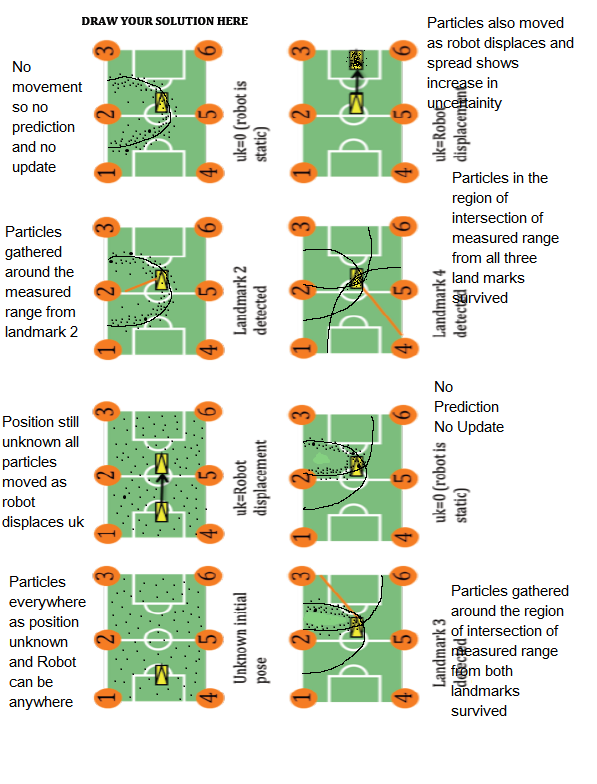
\includegraphics[width=0.7\textwidth]{solution2.png}

\label{Solution22}
\caption{Evolution of Particles}
\end{figure}
\begin{thebibliography}{9}
\bibitem{1}
$http://en.wikipedia.org/wiki/Image_segmentation$
\bibitem{2}
$http://en.wikipedia.org/wiki/Region_growing$
\end{thebibliography}
\end{document}

 
